% 本文件是示例论文的一部分
% 论文的主文件位于上级目录的 `main.tex`

\chapter{YOLO算法相关理论}

\section{YOLOv11网络结构}
YOLOv11的网络架构采用骨干网络-颈部网络-检测头的分层设计。骨干网络作为特征提取的基石,引入C3K2模块、SPPF(快速空间金字塔池化)和C2PSA(具有注意力机制的卷积模块)组件,实现了高效的底层特征提取;颈部网络将C2F模块替换为了C3K2模块,提升了特征聚合过程的整体性能,通过C2PSA模块增强了对空间注意力机制的关注;检测头负责生成目标检测和分类的最终预测,它处理从颈部网络传递过来的特征图,最终输出图像中目标的边界框和类别标签。\ref{fig:s}展示了YOLOv11的网络结构。
\begin{figure}[!htb]
  \centering
  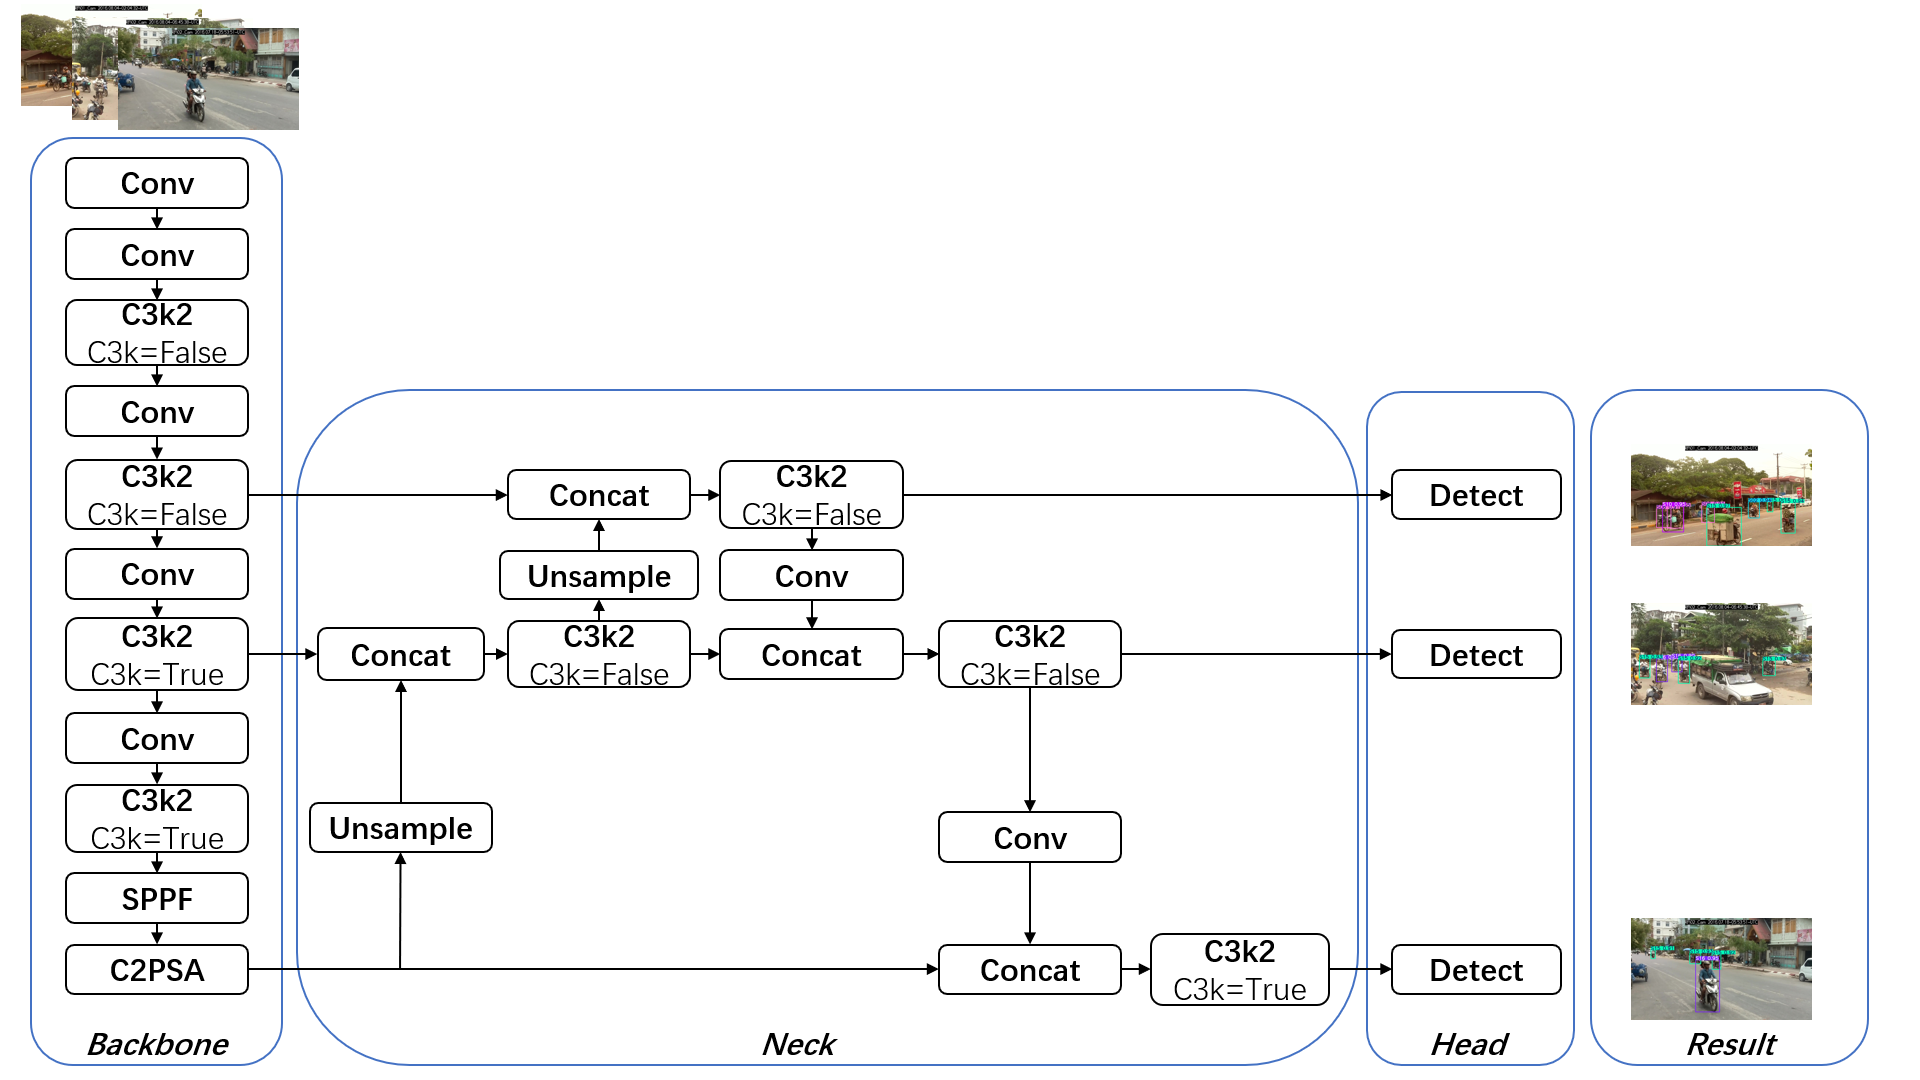
\includegraphics[width=1\textwidth]{figs/chap02/yolov11.png}
  \caption{YOLOv11网络模型}
  \label{fig:s}
\end{figure}

\subsection{骨干网络}
YOLOv11的骨干网络是整个架构的核心特征提取模块,包含Conv、C3K2、SPPF和C2PSA模块。

Conv卷积模块的处理步骤可以概括为数据准备、参数配置、卷积运算和非线性激活四步。Conv模块的输入通常是$(B, C, W, H)$四维张量,$B$表示训练批次;$C$表示数据通道数,彩色RGB图像的通道数为3;$W$表示图像的宽度,$H$表示高度。卷积层的核心参数包括卷积核、步长(stride)、填充(padding),卷积核决定特征提取的局部感知范围,步长控制卷积核滑动间隔以实现下采样,填充通过边界补零调整输出尺寸以及输出通道数。卷积运算这一步将配置好的卷积核应用于输入数据,通过滑动窗口对每个局部区域进行加权求和,实现特征提取。非线性激活应用ReLU、silu等激活函数引入非线性变换,使模型能够学习复杂模式,最终输出处理后的特征图用于后续层的计算。

C3K2模块是早期版本中引入的CSP(Cross Stage Partial) Bottleneck的演变,用来处理骨干网络不同阶段的特征提取。C3K2模块通过分割特征图,并应用一系列较小的(3×3)卷积核进行卷积操作,优化了网络中的信息流,这些卷积比较大的卷积核更快,计算成本更低。与YOLOv8的C2F模块相比,C3K2模块能够以更少的参数提升特征表示能力。
C3K2模块使用C3K模块来处理信息。它在开始和结束时各有一个Conv模块,中间是一系列的C3K模块。将起始Conv模块的输出与最后一个C3K模块的输出进行拼接,并以一个最终的Conv模块结束。这个模块借助CSP结构,致力于在速度和准确性之间保持平衡。
C3K模块的结构与C2F模块类似,但在此模块中不会进行分割操作。输入数据先经过一个卷积模块,随后经过一系列Bottleneck,并以最终的Conv块结束。这三个模块的结构如\ref{fig:c3k}所示。

\begin{figure}[!htb]
  \centering
  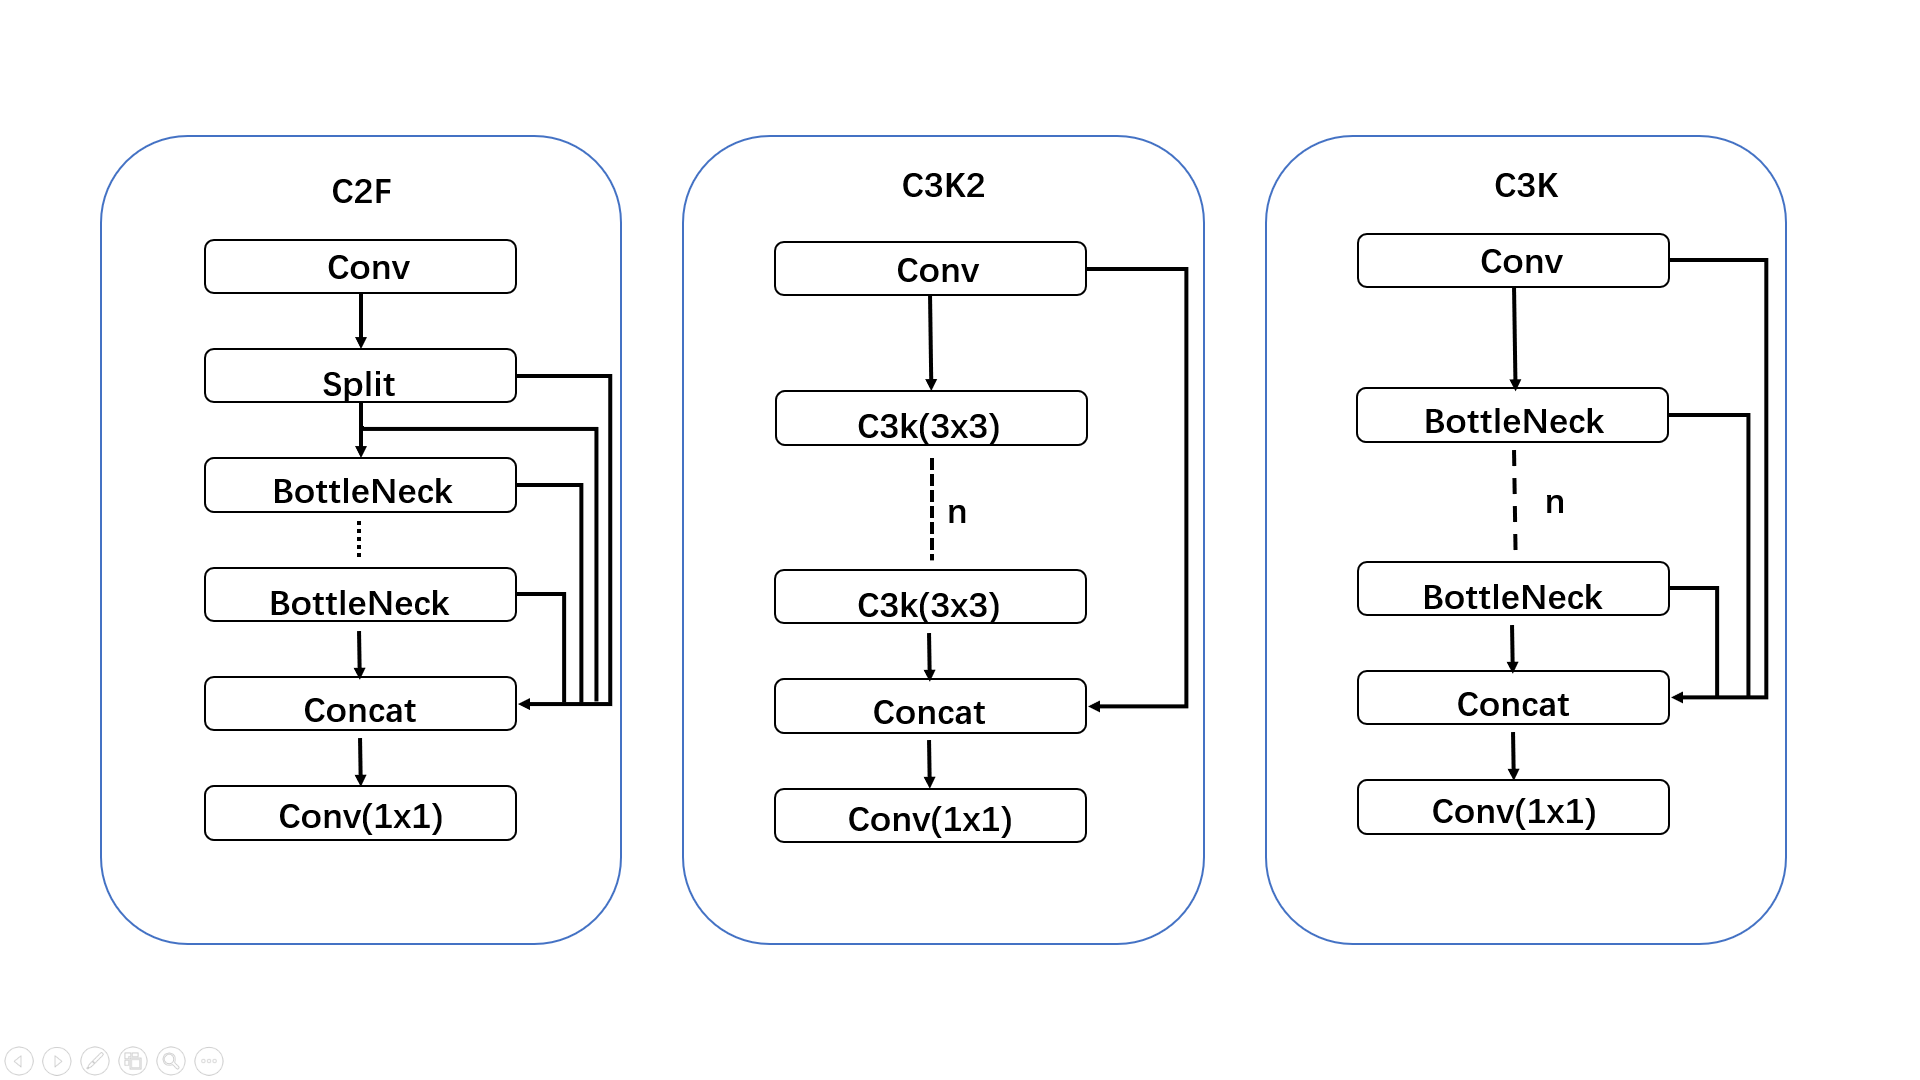
\includegraphics[width=0.9\textwidth]{figs/chap02/c2f.png}
  \caption{C2F和C3K2模块的比较}
  \label{fig:c3k}
\end{figure}

SPPF(Spatial Pyramid Pooling - Fast)模块是对SPP(Spatial Pyramid Pooling)模块的改进,主要用于增强模型对不同尺度目标的检测能力,其结构如\ref{fig:sppf}所示。SPPF模块接收C3K2模块输出的特征图,对特征图同时应用多个不同大小的最大池化操作(MaxPool),然后将原始特征图和所有池化后的特征图在通道维度上拼接,形成更丰富的多尺度特征表示,最后通过1×1卷积压缩拼接后的特征通道数,减少计算量。

\begin{figure}[!htb]
  \centering
  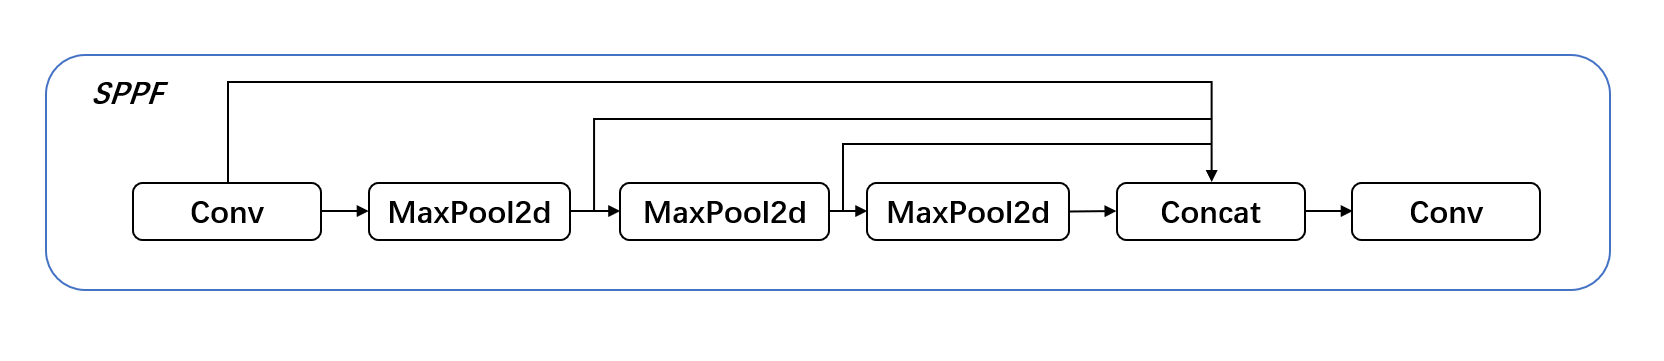
\includegraphics[width=0.9\textwidth]{figs/chap02/sppf.png}
  \caption{SPFF模块结构}
  \label{fig:sppf}
\end{figure}

该模块采用多尺度最大池化核进行特征提取,有效实现对目标多尺度特征的全面表征,通过对不同尺寸池化核获取的特征图进行整合。

C2PSA模块是YOLOv11的一大创新点,该模块结构如\ref{fig:c2psa}所示。此模块引入了注意力机制,提高模型对图像中重要区域(例如较小或部分遮挡的对象)的关注。C2PSA模块中的Position-Sensitive Attention封装了对输入张量应用位置敏感注意力和前馈网络的功能,提升了特征提取和处理能力。C2PSA模块采用两个PSA(Partial Spatial Attention)模块,分别处理特征图分支后再拼接,类似C2F模块结构。这种设置在兼顾计算成本与检测精度的同时,让模型聚焦空间信息,使YOLOv11在需关注物体细节以实现精确检测的场景中优于YOLOv8等版本。

\begin{figure}[!htb]
  \centering
  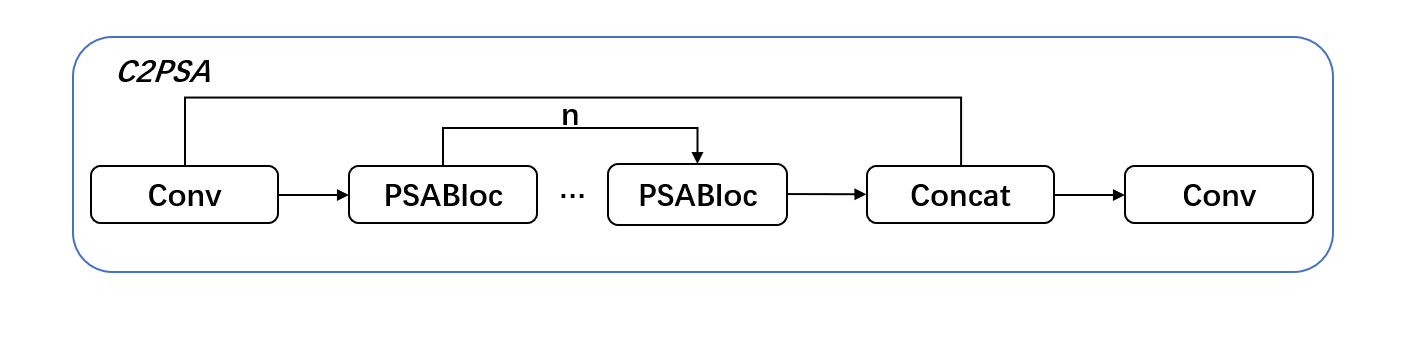
\includegraphics[width=0.9\textwidth]{figs/chap02/c2psa.png}
  \caption{C2PSA模块结构}
  \label{fig:c2psa}
\end{figure}

\subsection{颈部网络}
颈部网络由多个Conv卷积层、C3K2模块、Concat操作和上采样模块组成,并结合了C2PSA机制的优势。

Conv模块对特征图进行卷积运算,一方面可以调整特征图的通道数,使不同特征图在拼接前通道数匹配;另一方面能进一步提取特征,增强特征表达。C3K2模块应用了一系列较小的卷积核,以更少的参数提升特征表示能力。Concat模块沿着通道维度将多个特征图合并在一起,融合不同尺度的特征信息,增加特征的丰富度。
上采样模块通过运用插值等技术手段,实现特征图尺寸的扩充。这一操作的核心目的在于确保特征图维度与其他分支保持一致,借助这种方式,模型得以充分融合多尺度特征信息,提升了模型的检测精度。

颈部网络接收骨干网络不同层级输出的特征图,一些特征图会先经过Unsample上采样操作,使其尺寸与其他待拼接特征图一致,然后再进行Concat拼接。拼接后的特征图,再次经过若干C3K2模块和Conv卷积层,进一步融合与提炼特征。

\subsection{检测头}
与早期的YOLO版本类似,YOLOv11使用多尺度预测头来检测不同大小的对象。头部使用由主干网络和颈部网络生成的特征映射输出三种不同比例(低、中、高)的检测框。
检测头会输出来自三个特征映射(通常来自P3、P4和P5)的预测,对应于图像中的不同尺度级别。这种方法可以确保在更精细的细节(P3)中检测到较小的对象,而在更高级别的特征(P5)中捕获较大的对象​。

\section{YOLOv11损失函数}
YOLOv11的损失函数主要分为:边界框回归损失(BBox Loss)、分类损失(Classification Loss)和分布损失(Distribution Focal Loss, DFL)。

\subsection{边界框回归损失}
边界框回归损失函数为\ref{eq:bbox},$S$ 是网格的大小,
$B$ 是每个网格单元预测的边界框数量,
$1_{ij}^{obj}$ 表示第 $i$ 个网格单元中第 $j$ 个边界框是否负责预测目标。
$x, y$ 是边界框中心点的坐标。
$w, h$ 是边界框的宽度和高度。
$\lambda_{coord}$ 是权重系数,用于平衡不同部分的损失。

\begin{equation}
  \begin{aligned}
  \text{Box Loss} &= \lambda_{\text{coord}} \sum_{i = 0}^{S^2} \sum_{j = 0}^{B} \mathbb{1}_{ij}^{\text{obj}} \left( (x_i - \hat{x}_i)^2 + (y_i - \hat{y}_i)^2 \right) \\
  &+ \lambda_{\text{coord}} \sum_{i = 0}^{S^2} \sum_{j = 0}^{B} \mathbb{1}_{ij}^{\text{obj}} \left( (\sqrt{w_i} - \sqrt{\hat{w}_i})^2 + (\sqrt{h_i} - \sqrt{\hat{h}_i})^2 \right) \label{eq:bbox}
  \end{aligned}
\end{equation}

\begin{equation}
  \begin{aligned}
    (x_i - \hat{x}_i)^2 + (y_i - \hat{y}_i)^2 \label{eq:bbox_a}
  \end{aligned}
\end{equation}

\begin{equation}
  \begin{aligned}
    (\sqrt{w_i} - \sqrt{\hat{w}_i})^2 + (\sqrt{h_i} - \sqrt{\hat{h}_i})^2 \label{eq:bbox_b}
  \end{aligned}
\end{equation}

\ref{eq:bbox_a}衡量了预测边界框与真实边界框中心点之间的欧几里得距离平方。
\ref{eq:bbox_b}衡量了预测边界框与真实边界框的宽度和高度之间的差异。对宽度和高度取平方根减小了大尺寸边界框的影响,避免掩盖小尺寸边界框。

\subsection{分类损失}
分类损失函数见\ref{eq:cls},其核心作用是衡量模型对目标类别的预测准确性,并指导模型通过优化算法(如梯度下降)调整参数,从而提升分类性能。
\begin{equation}
  \begin{aligned}
    \text{Classification Loss} = \sum_{i = 0}^{S^2} \mathbb{1}_{i}^{\text{obj}} \sum_{c \in \text{classes}} (p_i(c) - \hat{p}_i(c))^2 \label{eq:cls}
  \end{aligned}
\end{equation}
$S$ 是网格的大小。
$1_{i}^{\text{obj}}$ 表示第 $i$ 个网格单元是否包含目标。
$p_i(c)$ 是模型预测的第 $i$ 个网格单元中目标属于类别 $c$ 的
$\hat{p}_i(c)$ 是真实的标签,表示第 $i$ 个网格单元中目标是否属于类别 $c$。
分类损失函数确保模型能正确识别图像中目标所属类别,最小化分类损失,使模型可处理多类别目标检测任务,提升模型分类准确性,助力模型学习类别特征差异,提高整体检测性能。


\subsection{分布损失}
目标检测领域普遍存在类别分布不平衡的现象,表现为特定类别的样本数量显著超过其他类别,这种数据分布失衡容易导致模型对高频类别表现出较好的识别性能,而对低频类别的检测准确率相对较低。分布损失函数用于优化模型在类别不平衡场景下的表现,其核心机制在于强化模型对困难样本的特征提取能力,从而显著提升对低频类别目标的检测效果。DFL损失函数公式为\ref{eq:dfl}。

\begin{equation}
  \begin{aligned}
    \text{DFL} = - \sum_{i = 1}^{N} \sum_{c = 1}^{C} y_{ic} \left( \alpha (1 - p_{ic})^{\gamma} \log(p_{ic}) + (1 - \alpha) p_{ic}^{\gamma} \log(1 - p_{ic}) \right) \label{eq:dfl}
  \end{aligned}
\end{equation}

$N$ 是样本数量。
$C$ 是类别的数量。
$y_{ic}$ 是第 $i$ 个样本的真实标签(one - hot 编码,只有一个元素为1,其余为0)。
$p_{ic}$ 是第 $i$ 个样本属于类别 $c$ 的预测概率。
$\alpha$ 是平衡因子,用于调整正负样本之间的权重。
$\gamma$ 是聚焦参数,用于控制对困难样本的关注程度。

% \section{YOLO各版本性能对比}
% YOLOv11与YOLOv9、YOLOv8等版本的性能对比见\ref{tab:yoloCompare}。mAP 50-95 这个指标衡量的是模型在IoU值从0.5到0.95范围内的平均精度,它的评价范围更加广泛。Speed CPU ONNX表示模型在CPU上基于ONNX推理时,处理一张图像所花费的时间,时间越短,说明模型在 CPU 上的推理效率越高,能够更快地给出检测结果。Speed T4 TensorRT10指模型在NVIDIA T4 TensorRT10硬件平台上进行推理时,处理一张图像所需的时间。Params表示模型的参数量,反映了模型的规模和复杂度,参数量越多,模型可学习的特征表示能力可能越强。FLOPs表示浮点运算量,它衡量了模型在进行一次前向传播(推理)过程中所执行的浮点运算次数,能体现出模型计算的复杂度。

% 从下表可以看出,对于同一版本的YOLO模型,规模越大的模型检测精度越高,但是速度会有所下降。对于同一对规模的YOLO模型,新版本的模型要比旧版本的模型检测精度高。YOLOv8相较于YOLOv5的同一规模的模型,检测速度更慢,但到了YOLOv11这里,同一规模的模型相较于之前的版本,检测速度都更快。即最新一代的YOLOv11,在提升了检测精度的同时,也加快了检测速度。

% \begin{table}[!htb]
%   \centering
%   \small % 缩小字体
%   \caption{YOLO各版本模型性能对比}
%   \label{tab:yoloCompare}
%   \begin{tabular}{ccccccccc}
%     \toprule
%     Model & \makecell{Size(pixels)} & \makecell{mAPval 50-95} & \makecell{Speed CPU \\ONNX(ms)} & \makecell{Speed T4 \\TensorRT10(ms)} & \makecell{Params \\(M)} & \makecell{FLOPs(B)} \\
%     \midrule
%     YOLOv5n & 640 & 34.3 & 73.6 & 1.06 & 2.6 & 7.7 \\
%     YOLOv5s & 640 & 43.0 & 120.7 & 1.27 & 9.1 & 24 \\
%     YOLOv8n & 640 & 37.3 & 80.4 & 0.99 & 3.2 & 8.7 \\
%     YOLOv8s & 640 & 44.9 & 128.4 & 1.2 & 11.2 & 28.6 \\
%     YOLOv9n & 640 & 38.3 & NA & NA & 2.0 & 7.7 \\
%     YOLOv9s & 640 & 46.8 & NA & NA & 7.2 & 26.7 \\
%     YOLOv11n & 640 & 39.5 & 56.1 & 1.5 & 2.6 & 6.5 \\
%     YOLOv11s & 640 & 47.0 & 90.0 & 2.5 & 9.4 & 21.5 \\
%     \bottomrule 
%   \end{tabular}
% \end{table}
% \begin{figure}[!htb]
%   \centering
%   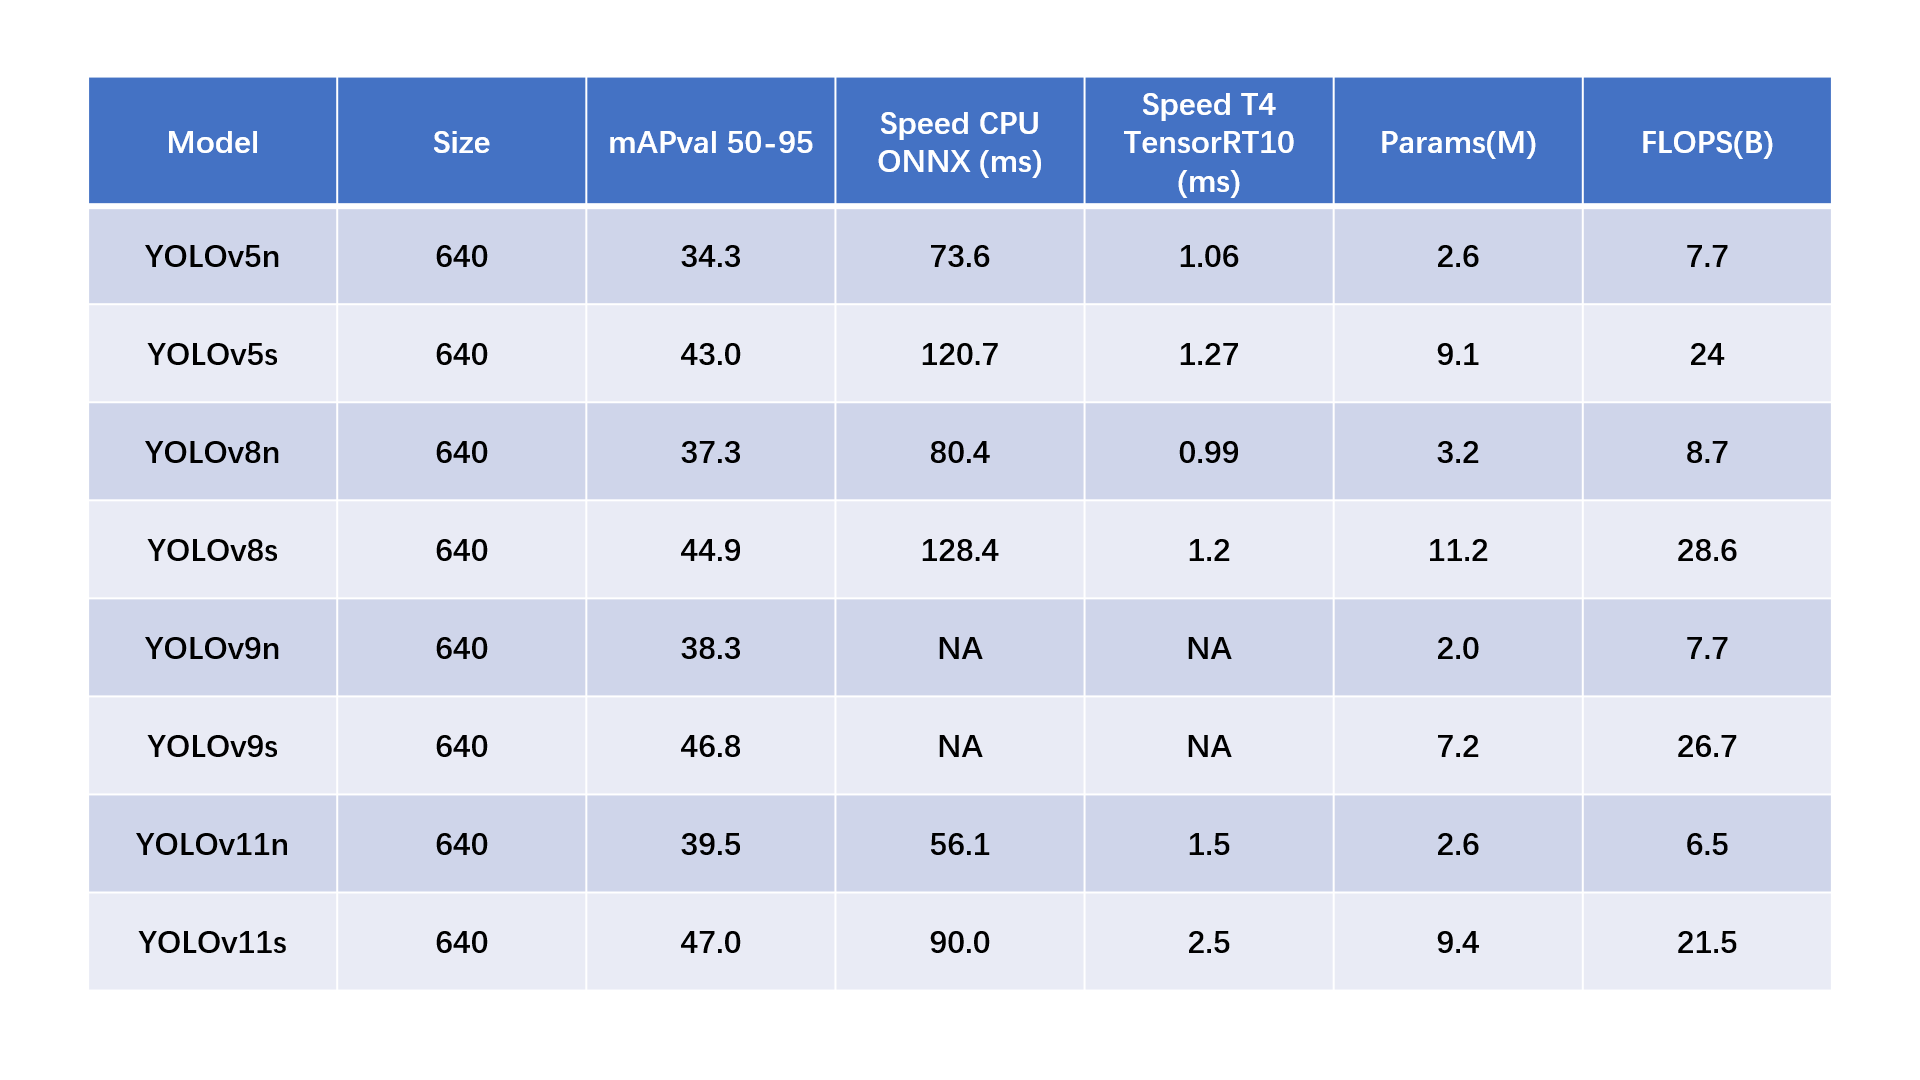
\includegraphics[width=0.85\textwidth]{figs/chap02/compare.png}
%   \caption{YOLO各版本模型性能对比}
%   \label{fig:compare}
% \end{figure}


\section{本章小结}
本章围绕YOLOv11算法相关理论展开,系统阐述了YOLOv11的网络结构,主要介绍了骨干网络、颈部网络和检测头,说明了YOLOv11对上述三个结构的改进点,并对YOLOv11中三个重要的损失函数做了详细的分析。


% \section{软件开发相关理论}
% 有了以上目标检测算法的支持,还需要开发一套图形化的界面方便用户使用。本系统采用前后端分离的方式进行开发,前端使用Vue框架,后端使用SpringBoot框架。下面将介绍一下SpringBoot和Vue框架,以及软件设计应遵循的基本原则。

% \subsection{后端框架SpringBoot}
% SpringBoot是一个基于Java语言的后端开发框架,它遵循 “约定优于配置” 的原则,使得开发人员可以将更多的精力放在业务逻辑的实现上,而不是花费大量时间写配置文件。它具有IOC(控制反转)和AOP(面向切面)两大特性:

% IOC是一种设计思想,它将对象的创建和管理从应用程序本身转移到一个外部容器(Spring 容器)中。在传统的软件开发中,对象之间的依赖关系通常由开发者在代码中直接进行创建和管理,这使得代码的耦合度较高,难以维护和扩展。而在SpringBoot中,通过IOC特性,对象只需声明其依赖关系,由Spring容器负责创建和注入这些依赖对象。这种特性使得各个组件可以独立开发、测试和维护,提高了代码的可复用性和可扩展性。通过IOC,当前组件只需要关心自己的业务逻辑,不需要关心他所依赖的组件的具体实现和创建过程。并且IOC容器能够实现一些无状态组件的复用,即单例Bean(SpringBoot中注入IOC容器的实例称为Bean),节约了服务器的内存。

% AOP 是一种编程范式,它允许将横切关注点从业务逻辑中分离出来,以一种非侵入式的方式对这些关注点进行统一处理。在 SpringBoot 中,AOP通过动态代理或字节码增强等技术,在运行时将切面逻辑织入到目标对象的方法执行过程中。SpringBoot的AOP默认使用动态代理来实现。如果目标对象实现了接口,Spring会使用JDK动态代理来创建代理对象;如果目标对象没有实现接口,Spring会使用CGLIB动态代理来创建代理对象。在运行时,当调用目标对象的方法时,实际上是调用代理对象的方法,代理对象会根据切入点和通知的定义,在方法执行前后或周围织入相应的切面逻辑。AOP特性使得业务逻辑代码更加清晰、简洁,易于理解和维护。当需要对横切关注点进行修改或扩展时,只需要在相应的切面中进行修改,而不需要在大量的业务逻辑代码中进行查找和修改,降低了代码的耦合度。

% 除了SpringBoot自身的一些特性,第三方的开源库也在日益拓展它的功能。在数据访问层面,有MyBatis、Redis等第三方库的支持,Spring Security在安全认证方面提供了强大的功能,Spring Cloud提供了微服务的基础功能。众多第三方开源库的贡献使得Spring Boot的功能不断丰富和完善,它不仅仅是一个应用搭建框架,而是成为了一个集数据访问、安全认证、微服务、消息通信、监控管理等功能与一体的庞大的开发生态。

% \subsection{前端框架Vue}
% JavaScript在Web开发领域扮演着核心角色,而Vue框架凭借其独特的设计理念和强大的功能,自诞生以来便迅速崛起,在众多框架中脱颖而出,成为了前端最热门的开发框架之一。Vue不仅为开发者提供了高效便捷的开发工具,还以简洁直观的语法降低了学习门槛,同时具备很好的性能和灵活性。

% 组件化是Vue框架的核心特性之一。在 Vue 开发中,界面被拆分为一个个独立且可复用的组件,每个组件都包含了自身的HTML、JavaScript和CSS,形成一个高度内聚的代码单元。这种组件化的开发模式不仅使代码结构清晰明了,便于开发者理解和维护,还极大地提高了代码的复用性。

% Vue的响应式机制实现了数据与页面DOM结构的双向绑定,当应用中的数据状态发生改变时,与之关联的视图内容会自动触发更新,与传统的直接操作 DOM节点进行页面更新的方式不同,Vue开发者无需手动操作DOM,仅需专注于数据逻辑处理,极大简化了开发者的工作。

% \subsection{软件设计的基本原则}
% 下面介绍软件设计的基本原则,包括高内聚低耦合、开闭原则、设计模式以及领域驱动设计。本系统在代码实现层面也运用了领域驱动思想来搭建系统架构,遵循开闭原则,通过设计模式降低系统耦合度,提升系统的可维护性和拓展性。
% \subsubsection{高内聚低耦合}
% 高内聚指一个模块内各个元素之间的联系紧密,它们共同完成一个相对独立且明确的功能。例如,在一个音乐播放软件中,负责音乐播放功能的模块,其内部包含的加载音乐文件、控制播放进度、调整音量等功能元素都紧密围绕音乐播放这一核心功能,相互协作来实现完整的音乐播放流程。这种模块功能单一明确,开发人员能够快速了解模块的作用和功能逻辑,降低了对软件系统整体理解的难度。并且,对某个功能进行修改或优化时,由于相关的功能元素都集中在一个模块内,开发人员可以在该模块内进行针对性的修改,而不用担心影响到其他不相关的功能。

% 低耦合强调模块与模块之间的相互依赖关系要尽可能少,模块之间的接口要简单、清晰。比如,在一个电商系统中,用户管理模块和商品推荐模块是两个不同的模块,用户管理模块主要负责用户的注册、登录、信息修改等功能,商品推荐模块则根据用户的浏览历史和购买行为为用户推荐商品。这两个模块之间通过简单的接口进行交互,不涉及对方模块的内部实现细节。当需要对系统进行功能扩展时,由于模块之间耦合度低,新增的功能模块对现有模块的影响较小,能够更容易地集成到系统中。例如,在上述电商系统中,如果要增加一个促销活动模块,由于它与用户管理模块和商品推荐模块的耦合度低,只需要通过定义好的接口与其他模块进行交互即可,不会对其他模块的内部结构和功能造成太大的改变。模块之间的低耦合使得它们相对独立,一个模块的故障或修改不太容易传播到其他模块,从而提高了整个系统的稳定性和可靠性。

% \subsubsection{开闭原则}
% 软件实体(类、模块、函数等)应该对扩展开放,对修改关闭。这意味着当软件系统需要添加新功能时,应该通过扩展现有代码来实现,而不是直接修改已有的代码。这样可以避免对源代码的入侵,提高了系统的稳定性。可以通过抽象和多态、依赖注入以及设计模式来遵循开闭原则。

% \subsubsection{设计模式}
% 当软件系统规模变大时,如果没有良好的设计模式,代码可能会变得混乱不堪,难以理解和修改。而采用设计模式,代码结构更加清晰,各个模块的职责明确,维护起来更加容易。随着业务的发展,软件系统需要不断添加新功能。设计模式使得软件具有更好的扩展性,能够轻松应对这些变化。

% \subsubsection{领域驱动设计}
% 领域驱动设计(Domain-Driven Design,DDD)是一种用于开发复杂业务系统的软件设计方法,将软件设计的重点放在领域模型上,即对业务领域的概念、规则和流程进行抽象和建模。本系统也参照领取驱动设计的思想去做领域划分,搭建系统架构。
% DDD通过将业务领域划分为不同的限界上下文和聚合,使得软件系统的结构更加清晰,模块之间的耦合度降低。当业务需求发生变化时,能够更方便地定位和修改相关的领域模型和代码,而不会对整个系统造成太大的影响,提高了软件的可维护性和可扩展性。在访问第三方API时,DDD主张用防腐层隔离自身系统和第三方接口,这里的防腐层不仅可以作为一个适配器,去对接本系统和第三方的接口,还可以将第三方的腐化隔离在外,即自身系统不会因为第三方系统的崩溃而不可用。

% \begin{table}[htbp]
%   \centering
%   \caption{YOLO模型性能对比}
%   \begin{tblr}{
%     colspec = {lcccccc},
%     hline{1,Z} = {1pt, solid},
%     hline{2} = {solid},
%     cells = {font=\small}
%   }
%   Model & Size (pixels) & mAPval 50 - 95 & Speed CPU ONNX (ms) & Speed T4 TensorRT10 (ms) & Params (M) & FLOPs (B) \\
%   \midrule
%   YOLOv5n & 640 & 34.3 & 73.6 & 1.06 & 2.6 & 7.7 \\
%   YOLOv5s & 640 & 43.0 & 120.7 & 1.27 & 9.1 & 24 \\
%   YOLOv8n & 640 & 37.3 & 80.4 & 0.99 & 3.2 & 8.7 \\
%   YOLOv8s & 640 & 44.9 & 128.4 & 1.2 & 11.2 & 28.6 \\
%   YOLOv9n & 640 & 38.3 & NA & NA & 2.0 & 7.7 \\
%   YOLOv9s & 640 & 46.8 & NA & NA & 7.2 & 26.7 \\
%   YOLOv11n & 640 & 39.5 & 56.1 & 1.5 & 2.6 & 6.5 \\
%   YOLOv11s & 640 & 47.0 & 90.0 & 2.5 & 9.4 & 21.5 \\
%   \end{tblr}
% \end{table}
% 作为深度学习算法的关键基石,神经网络(Neural Network),又称人工神经网络,其构建理念来自于人类大脑的神经元。人类大脑的神经元通过突触连接,形成复杂网络实现信息传递与处理。神经网络借鉴这一生物机制,构建出由大量人工神经元组成的计算模型。这些人工神经元模拟生物神经元接收、处理和传递信号的过程,通过数据驱动的方式,不断调整神经元之间的连接权重,进而从海量数据中学习规律与模式,逐步积累 “经验”。

% \section{神经网络模型}
% 经网络中的神经元就像一个个微小的信息处理单元,它们通过权重相互连接,形成了一个复杂的网络结构。输入层负责接收外部数据,将数据传递给隐藏层。隐藏层可以有多个,它们对输入数据进行层层处理和特征提取。每个隐藏层中的神经元会接收上一层神经元的输出作为输入,并根据连接权重对这些输入进行加权求和,再经过激活函数处理后,将结果传递给下一层。输出层则根据隐藏层的处理结果,输出最终的预测或分类结果。随着网络深度的增加,神经网络理论上可以学习到更复杂的特征和模式,但同时也会带来训练时间长、容易过拟合等问题。

% \begin{figure}[!htb]
%   \centering
%   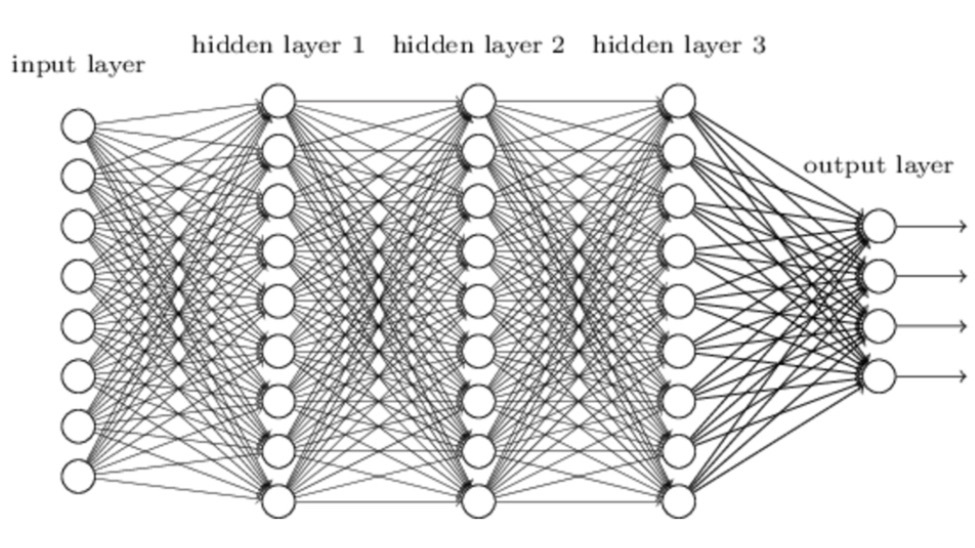
\includegraphics[width=0.6\textwidth]{figs/chap02/image.png}
%   \caption{神经网络模型}
%   \label{fig:DDN}
% \end{figure}

% 在神经网络中,神经元之间的连接关系十分复杂。一个神经元的输出往往会作为多个神经元的输入,这种多对多的连接方式使得信息能够在网络中广泛传播和共享。比如在图像分类任务中,某个神经元在提取图像的边缘特征后,其输出会被传递到多个负责更高级特征提取的神经元中,这些神经元会结合其他输入信息,进一步提取图像的形状、纹理等更复杂的特征。同时,一个神经元的输入也可能由多个神经元的输出构成,这使得神经元能够综合多方面的信息进行处理。这种复杂的连接方式,让神经网络能够模拟出高度复杂的非线性关系,从而实现对各种复杂数据的处理和分析。

% 以图像分类、目标检测等深度学习任务为例,首先需要对大量图像进行标注,标注内容包括图像中目标的类别、位置等信息。这些标注过的图像被作为训练数据输入到神经网络中。在训练过程中,神经网络会根据当前的模型参数,对输入图像进行前向传播计算,得到输出值。这个输出值会与标注的真值进行比对,通过损失函数计算两者之间的差异。损失函数用于衡量模型预测结果与真实结果之间的差距,常见的损失函数有交叉熵损失函数、均方误差损失函数等。接下来,通过反向传播算法,根据损失函数的结果,从输出层向输入层反向传播误差,计算出每个神经元连接权重的梯度。梯度表示了损失函数对权重的变化率,通过梯度下降法等优化算法,根据梯度来调整模型参数,使得损失函数的值逐渐减小。这个过程不断重复,直到模型参数收敛,即损失函数的值不再下降或下降非常缓慢,此时模型达到正常拟合的程度。在这个过程中,“自监督式学习” 是一种重要的训练方式,它通过利用数据本身的结构和特征来生成监督信号,而不需要额外的人工标注。例如,在图像自监督学习中,可以通过对图像进行旋转、裁剪等变换,让神经网络学习如何恢复原始图像,从而学习到图像的特征和模式。这种学习方式可以充分利用大量未标注数据,提高模型的泛化能力和性能。

% \section{卷积神经网络}

% 卷积神经网络(CNN)是一种专门为处理具有网格结构数据(如图像、音频)而设计的深度学习模型,其结构主要包括输入层、卷积层、池化层、全连接层。

% \begin{figure}[!htb]
%   \centering
%   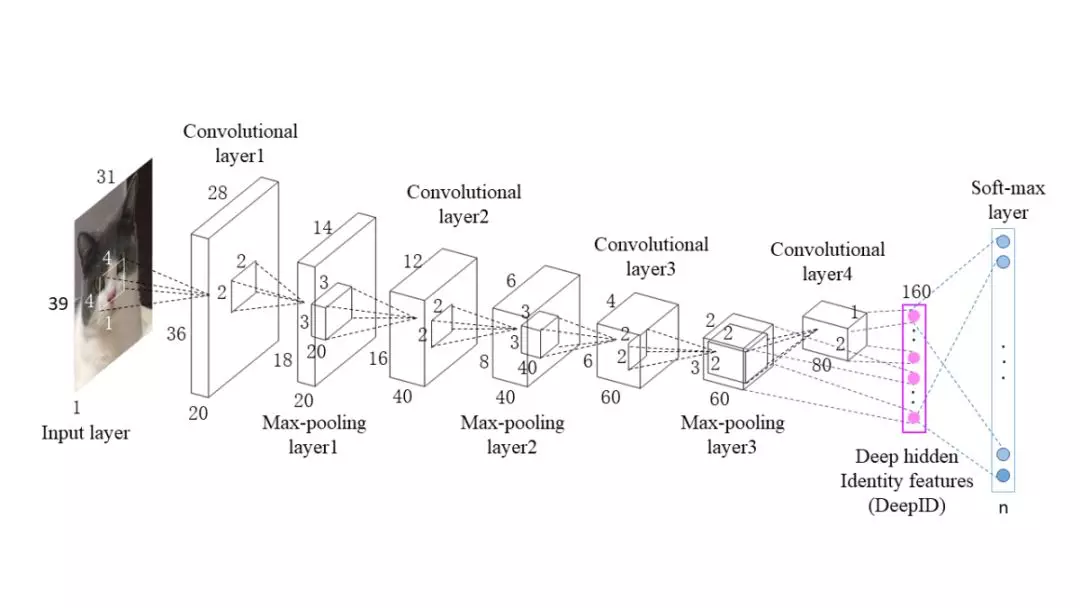
\includegraphics[width=0.85\textwidth]{figs/chap02/CNN.png}
%   \caption{卷积神经网络结构}
%   \label{fig:CNN}
% \end{figure}

% \subsection{输入层}
% 主要负责将原始数据输入到网络中。对于图像数据,通常会将图像的像素值作为输入,其维度一般为三维,分别表示图像的高度、宽度和通道数,即w * h * d,其中对于图片输入来说通常是以RGB三通道的形式输入,所以d通常是3。

% \begin{figure}[!htb]
%   \centering
%   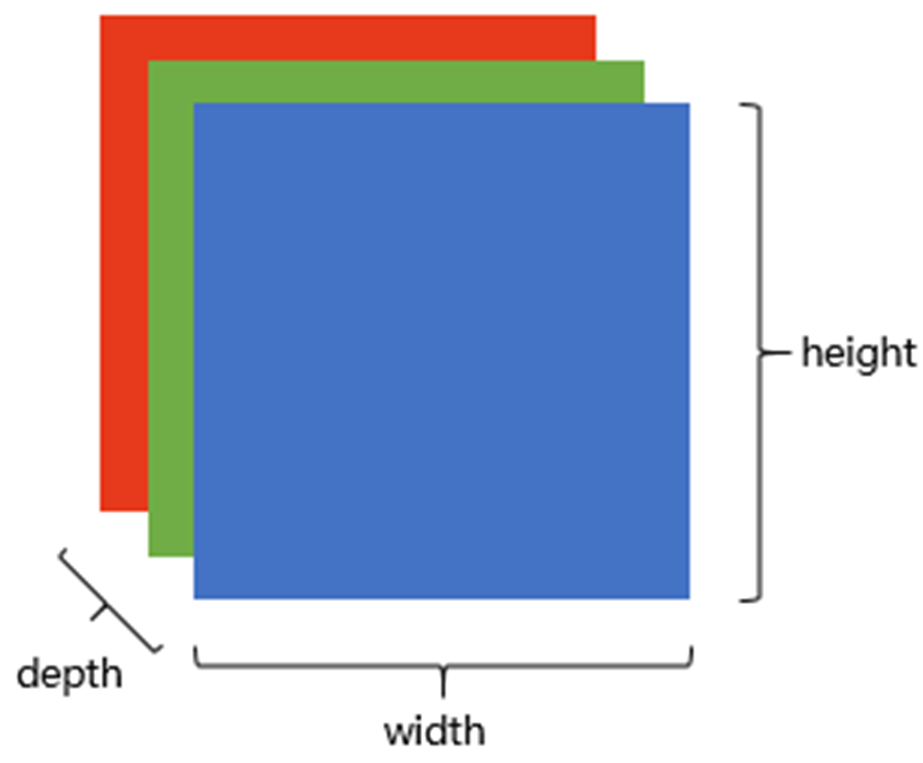
\includegraphics[width=0.4\textwidth]{figs/chap02/input.png}
%   \caption{输入图像}
%   \label{fig:input}
% \end{figure}

% \subsection{卷积层}
% \subsubsection{卷积核}
% 卷积核是一个小的二维矩阵,也被称为滤波器。它在输入数据上滑动,通过与对应位置的元素进行乘法和求和运算,实现对输入数据的特征提取。卷积核的尺寸通常远小于输入数据的尺寸,常见的有 3×3、5×5等。较小的卷积核可以减少计算量和模型参数数量,同时也能更好地捕捉局部特征。

% \subsubsection{步长}
% 在进行卷积操作时,卷积核会在输入数据上以一定的步长滑动。步长表示卷积核在每次移动时的距离。例如,步长为1表示卷积核每次移动一个像素点;步长为2则表示每次移动两个像素点。较大的步长可以减少计算量和输出特征图的尺寸,但可能会丢失一些细节信息;较小的步长则可以更细致地提取特征,但计算量会增加。

% \subsubsection{填充}
% 为了控制输出特征图的尺寸和保留图像边缘的信息,通常会在输入数据的边缘添加额外的行和列,这一操作称为填充。常用的填充方式有零填充,即将边缘添加的元素设置为 0。例如,对于一个 5×5 的输入图像,使用 3×3 的卷积核进行卷积操作,如果不进行填充,输出特征图的尺寸会变小;而进行适当的填充后,可以使输出特征图的尺寸与输入图像相同,从而更好地保留图像的整体信息。

% \subsection{池化层}
% 池化层主要用于对卷积层输出的特征图进行下采样,以减少数据量和模型的计算量,同时保留重要的特征信息。

% \subsubsection{最大池化}
% 在每个池化窗口内,取该窗口内特征值的最大值作为池化结果。例如,对于一个2×2的池化窗口,在窗口覆盖的区域中选择最大的数值作为该窗口的输出。这种方式能够突出图像中的显著特征,因为最大值通常对应着图像中最强烈的响应区域,如边缘、角点等。最大池化在保留图像的纹理和细节特征方面表现较好。
% \subsubsection{平均池化}
% 计算每个池化窗口内特征值的平均值作为池化结果。与最大池化不同,平均池化更注重保留图像的整体信息,它对特征图进行平滑处理,减少了局部噪声的影响。在一些对图像整体特征较为敏感的任务中,平均池化可能会有较好的效果。

% \begin{figure}[!htb]
%   \centering
%   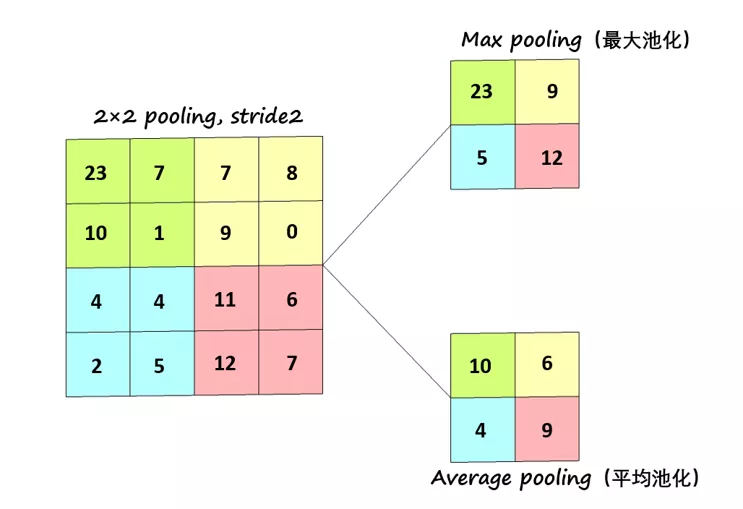
\includegraphics[width=0.6\textwidth]{figs/chap02/pooling.png}
%   \caption{最大池化和平均池化}
%   \label{fig:pooling}
% \end{figure}

% \subsection{全连接层}
% 全连接层其中的每个神经元都与上一层的所有神经元相连,通过权重和偏置对输入进行线性变换,并经过激活函数引入非线性。它的作用是整合特征,将前面层提取的特征进行综合,以用于分类或其他预测任务,在模型训练中通过调整大量参数来学习复杂的函数关系。
